\setcounter{chaptercntr}{4}

\sectionbreak {
\gostTitleFont
\redline
\thechaptercntr . 
РАЗРАБОТКА, ОБУЧЕНИЕ И ОЦЕНКА МОДЕЛИ НЕЙРОННОЙ СЕТИ
}


\titlespace

\subsection*{ 
  \gostTitleFont
  \redline
  \thechaptercntr .\thesubchaptercntr \spc 
  Выбор архитектуры нейронной сети для прогнозирования
} \addtocounter{subchaptercntr}{1} 

\subtitlespace

{\gostFont

  \par \redline Для выбора архитектуры нейронной сети необходимо для начала понять, какие архитектуры используются для прогнозирования данных временных рядов. Зачастую для выполнения данной задачи используются однослойные персептроны, многослойные персептроны и рекуррентные нейронные сети. Обращая внимание на свойства данных, становится понятно, что однослойный персептрон не сможет обеспечить необходимую обобщающую способность. Тогда остаётся выбор между многослойным персептроном и рекуррентной нейронной сетью. 
  
  \par \redline Относительно многослойных персептронов существует теорема, согласно которой персептрон с одним скрытым слоем является универсальным аппроксиматором, т. е. он способен с любой степенью точности аппроксимировать любую непрерывную функцию, если в качестве функции активации нейронных элементов скрытого слоя используется непрерывная, монотонно возрастающая, ограниченная функция. При этом точность аппроксимации функции зависит от количества нейронов в скрытом слое. Чем больше количество нейронов, тем больше точность аппроксимации. Однако при слишком большой размерности скрытого слоя может наступить явление, которое называется перетренировкой сети, когда сеть имеет плохую обобщающую способность.  

  \par \redline Что касается RNN, также существует теорема, говорящая нам о том, что любая нелинейная динамическая система при использовании достаточного количества сигмоидальных нейронных элементов в скрытом слое с любой точностью может быть аппроксимирована рекуррентной нейронной сетью. 

  \par \redline Выходит, что для прогнозирования можно использовать как многослойный персептрон, так и RNN. Однако, RNN обладает очень интересной чертой: она обладает, так называемой, памятью, способной <<запоминать>> особенности данных временных рядов. Такой памятью многослойный персептрон не обладает. Поскольку данные имеют в себе отличающиеся друг от друга, но повторяющиеся в будущем участки, то наличие такой памяти было бы очень кстати. Также, как можно будет узнать дальше, большинство, если не все, RNN имеют чётко определённую структуру, в которую довольно сложно что-то добавить, да и нет в этом необходимости. В случае с многослойными персептронами, их структура не постоянна: необходимо подбирать количество скрытых слоёв. Поэтому в некотором смысле, реализация RNN не только будет выгоднее, но и проще. При этом, если обратиться к Kaspersky MLAD, то можно вспомнить, что для прогнозирования данных телеметрии используются именно RNN. Учитывая всё вышенаписанное, выбор архитектуры падает на RNN.

  \par \redline Теперь необходимо выбрать модель RNN. Существует большое количество различных рекуррентных нейронных сетей: SRN Джордана, SRN Элмана, мультирекуррентная нейронная сеть, LSTM, GRU и так далее. Однако, одной из самых распространённых и эффективных RNN считают LSTM сеть. Эта сеть встречается куда чаще, чем её модификации, такие как GRU, MGU, LSTM <<с глазками>> и другие. Основной задачей ставилось упрощение сети без вреда её точности, результатом чего появилась ранее упомянутая GRU, точность предсказаний которой не уступает LSTM, но при этом сеть менее громоздкая. Упростить удалось и GRU, получив тем самым MGU, однако точность этой сети всё также сравнивалась с LSTM. Поэтому для данной работы за основу будет взята классическая LSTM.

  \par \redline К слову, LSTM была выбрана и Kaspersky при разработке системы MLAD. Это в очередной раз говорит о популярности и надёжности сети LSTM, что укрепляет уверенность в выборе LSTM сети для данной работы. 

  \par
}

\subtitlespace

\subsection*{ 
  \gostTitleFont
  \redline
  \thechaptercntr .\thesubchaptercntr \spc 
  Обзор LSTM как средства прогнозирования
} \addtocounter{subchaptercntr}{1} 
  
\subtitlespace
  
{\gostFont

  \par \redline Сеть LSTM обладает двумя видами памяти, которые способны сохранять различные зависимости в данных. Есть долгосрочная память, которая обозначается как $ C_{t} $, и краткосрочная память, которая обозначается как $ H_{t} $. Как можно догадаться, долгосрочная память сети хранит в себе особенности данных на протяжении всей истории, а краткосрочная память хранит зависимости ближайших промежутков и сильнее влияет на результат прогноза. Зачастую краткосрочную память сети обозначают как её выход. При этом входом сети является некоторый вектор данных, на основании которых будет делаться прогноз. Вектор входных данных будет обозначаться как $ X_{t} $. Как можно заметить, у всех параметров сети присутствует временная компонента t. Это говорит о том, что расчёт прогноза происходит относительно времени. Каждая новая итерация сети происходит с изменением времени. Память сети изменяется на одной из итерации и передаётся на следующую, тем самым сеть и сохраняется особенности данных временного ряда, который был подан на вход сети. Такая передача памяти возможно благодаря, так называемых в нейронных сетях, обратных связях, наличие которые и определяет сеть как рекуррентную. Вышеописанное можно увидеть на рисунке \thechaptercntr .\theimagecntr. 

  \begin{figure}[H]
    \centering
    \def\svgwidth{\textwidth}
    \includesvg[width=200pt]{images/LSTMBlackBox.svg}
    \caption*{\gostFont Рисунок \thechaptercntr .\theimagecntr \spc {--} Блок LSTM сеть с изображением обратных связей.}
    \label{fig:LSTMBlackBox}
  \end{figure} \addtocounter{imagecntr}{1}

  \par \redline Каждый такой блок сети LSTM, изображённый на рисунке выше, зачастую называют ячейкой LSTM. Связь этих ячеек между собой можно гораздо лучше увидеть на развёрнутой схеме LSTM, изображённой на рисунке \thechaptercntr .\theimagecntr. 

  \begin{figure}[H]
    \centering
    \def\svgwidth{\textwidth}
    \includesvg[width=\textwidth]{images/LSTMSequence.svg}
    \caption*{\gostFont Рисунок \thechaptercntr .\theimagecntr \spc {--} Взаимосвязь ячеект LSTM в развёрнутом виде.}
    \label{fig:LSTMSequence}
  \end{figure} \addtocounter{imagecntr}{1}

  \par \redline Теперь необходимо изучить саму ячейку LSTM. Её структура представлена на рисунке \thechaptercntr .\theimagecntr. Говоря о LSTM, можно встретить специальную лексику, которая относится к описанию этой сети. К специальной лексике относятся такие понятия как: врата забывания ($F_t$), врата входа ($I_t$), врата новой памяти ($G_t$), врата выхода ($O_t$), долгосрочная память сети ($C_t$) и краткосрочная память сети ($H_t$). Разберём каждый из этих понятий по отдельности, параллельно определяя формулы, по которым можно их рассчитать.

  \begin{sidewaysfigure}
    \centering
    \def\svgwidth{\textwidth}
    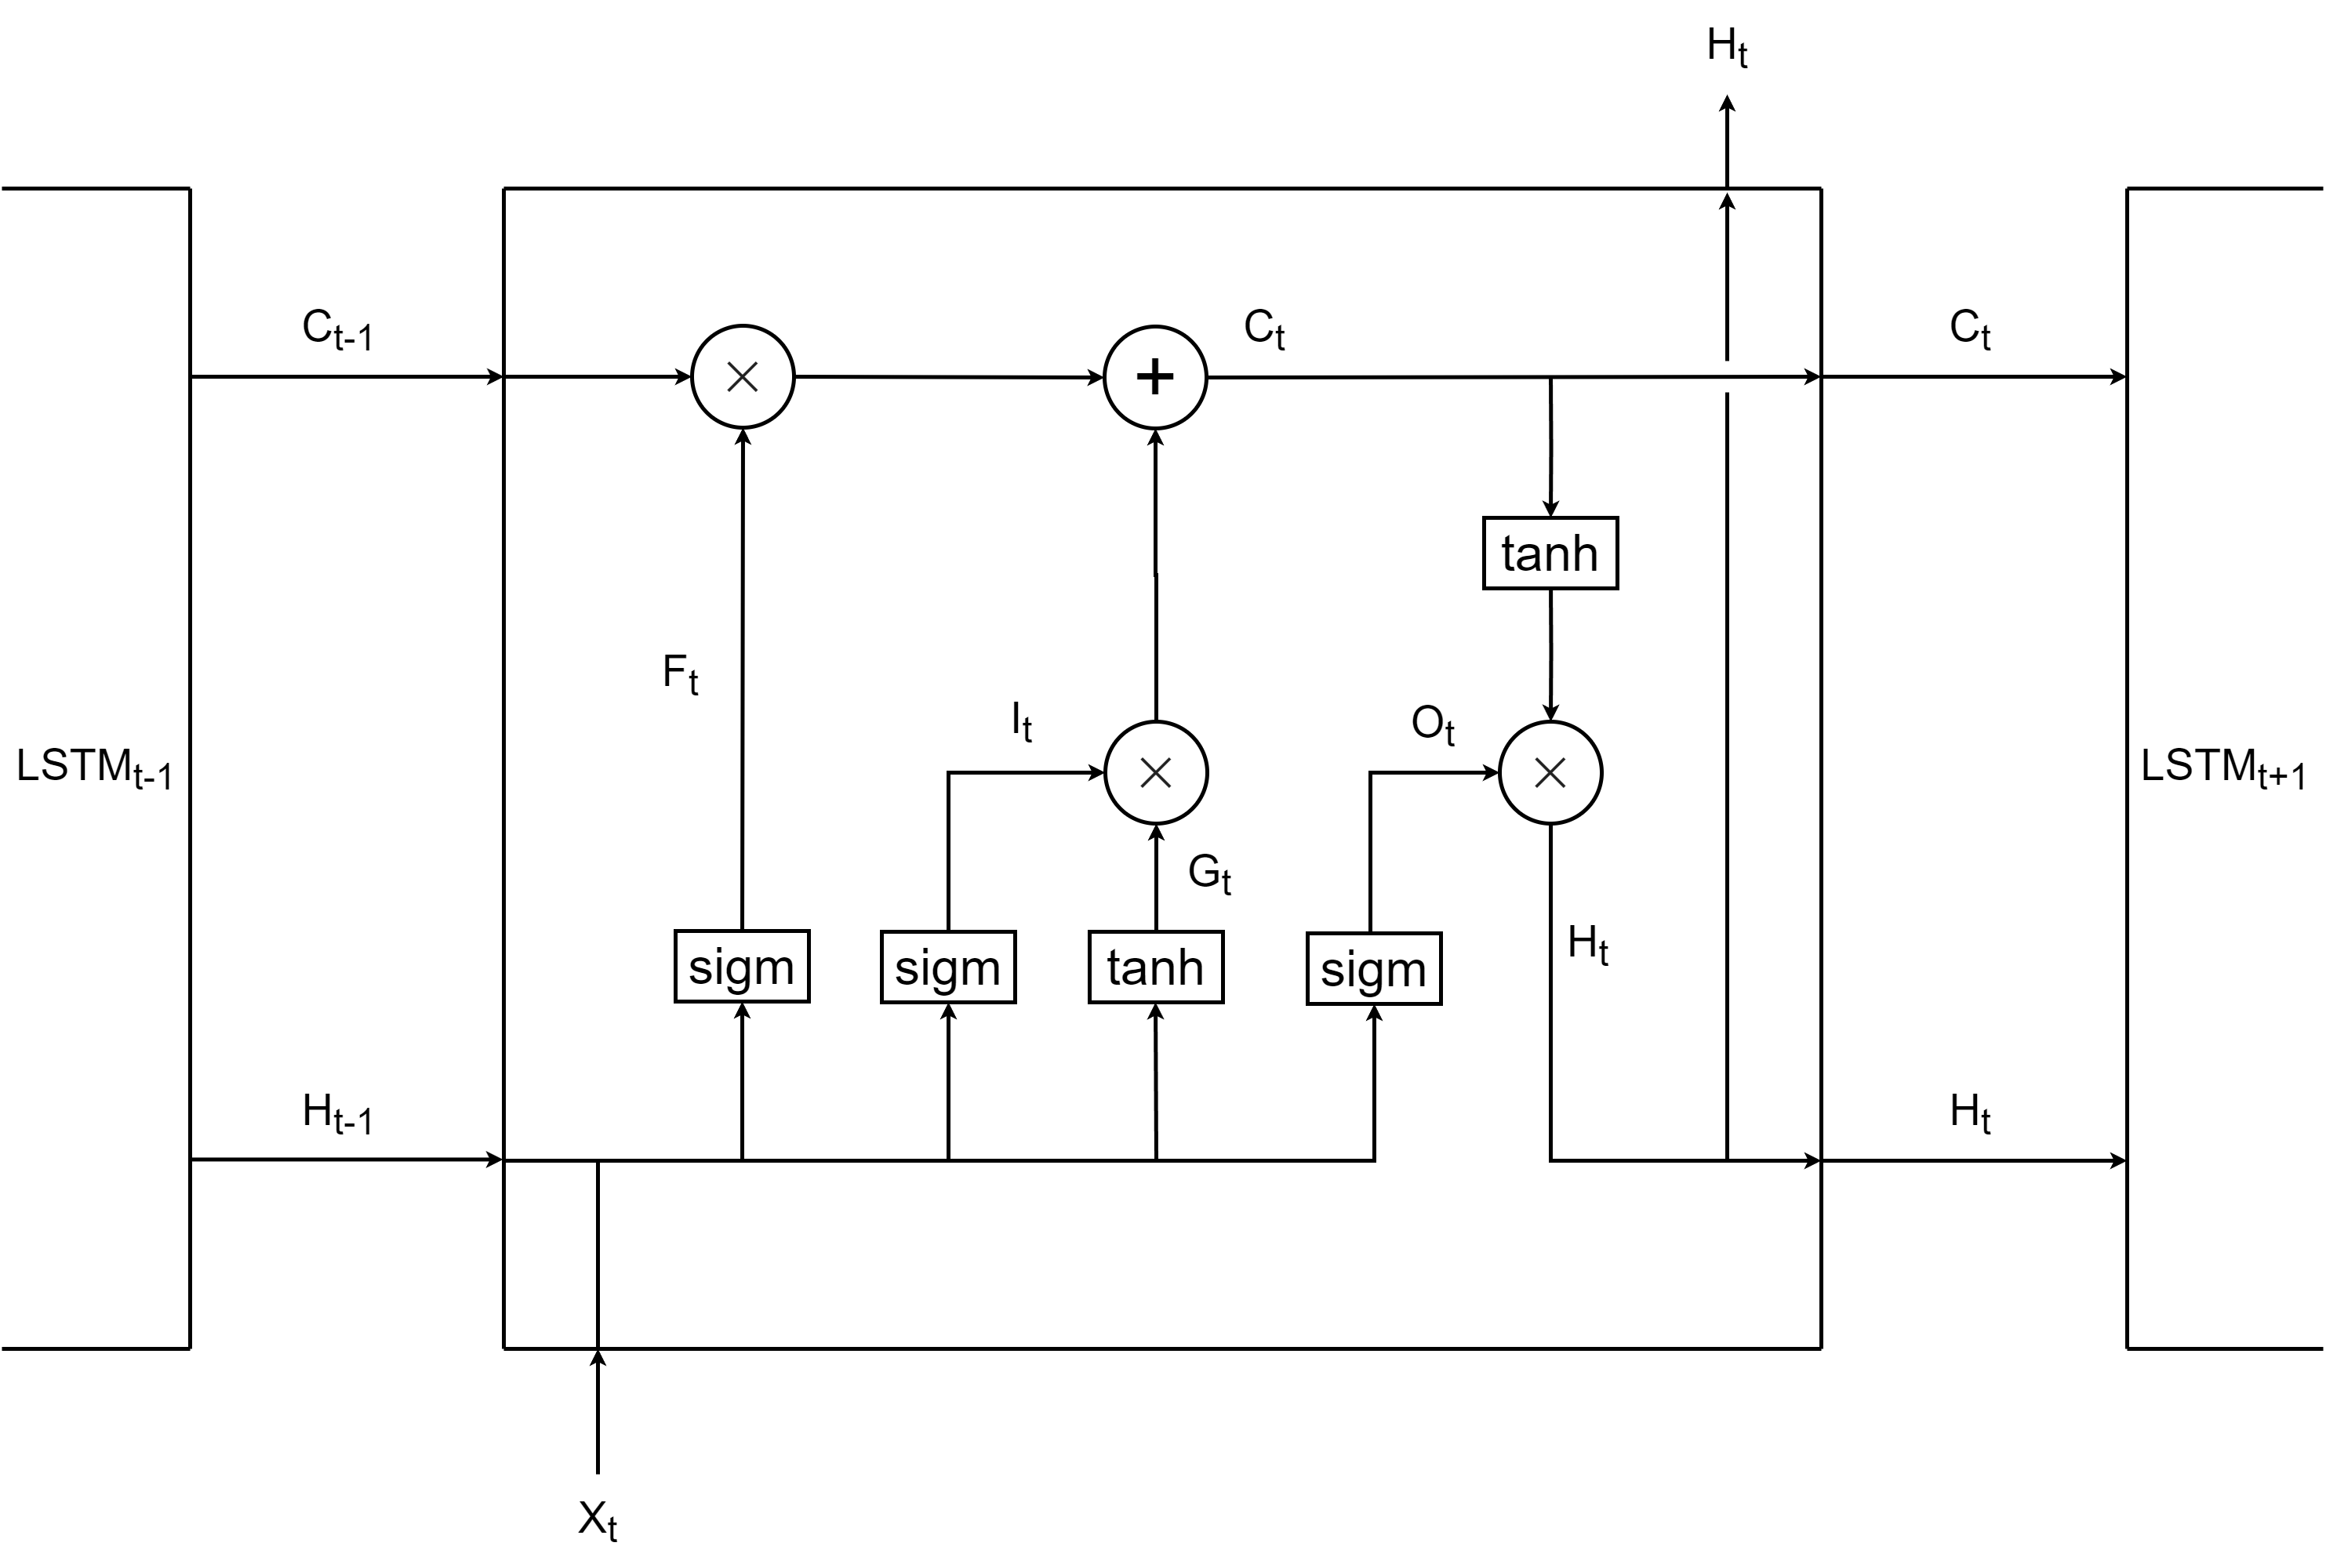
\includegraphics[scale=0.225]{../GMs/Pl3/LSTM.png}
    \caption*{\gostFont Рисунок \thechaptercntr .\theimagecntr \spc {--} Структура ячейки LSTM.}
    \label{fig:LSTM}
  \end{sidewaysfigure} \addtocounter{imagecntr}{1}

  \par \redline Врата забывания ($F_t$) необходимы для исключения некоторый информации из долгосрочной памяти сети ($C_t$), которую нужно <<забыть>>, отсюда и название врат, и рассчитываются по формуле (\thechaptercntr .\theformulacntr):

  \formulaspace \par \redline 
    $F_t = sigm(W_f \times X_t + U_f \times H_{t-1} + b_f)$
    \hfill (\thechaptercntr .\theformulacntr) \redline
  \formulaspace \addtocounter{formulacntr}{1}

  \begin{tabular}{p{0,875cm}p{0,3cm}p{15,175cm}}
		& где  & $F_t$ {--} вектор врат забывания; \\
    & 	   & $X_t$ {--} вектор входных значений; \\
		& 	   & $W_f$ {--} матрица весов врат забывания для взаимодействия с входным вектором; \\
    & 	   & $H_{t-1}$ {--} вектор краткосрочной памяти сети на прошлой итерации (из прошлого); \\
    & 	   & $b_f$ {--} вектор смещения для врат забывания; \\
    & 	   & $U_f$ {--} матрица весов врат забывания для взаимодействия с вектором краткосрочной памяти. \\
  \end{tabular}

  \par \redline Врата новой памяти ($G_t$) отвечают за формирование, так скажем, претендентов, которые должны стать частью новой долгосрочной памятью сети ($C_t$), и рассчитываются по формуле (\thechaptercntr .\theformulacntr):

  \formulaspace \par \redline 
    $G_t = tanh(W_g \times X_t + U_g \times H_{t-1} + b_g)$
    \hfill (\thechaptercntr .\theformulacntr) \redline
  \formulaspace \addtocounter{formulacntr}{1}

  \begin{tabular}{p{0,875cm}p{0,3cm}p{15,175cm}}
		& где  & $G_t$ {--} вектор врат новой памяти; \\
		& 	   & $W_g$ {--} матрица весов врат новой памяти для взаимодействия с входным вектором; \\
    & 	   & $b_g$ {--} вектор смещения для врат новой памяти; \\
    & 	   & $U_g$ {--} матрица весов врат новой памяти для взаимодействия с вектором краткосрочной памяти. \\
  \end{tabular}

  \par \redline Врата входа ($I_t$) решают, что из врат новой памяти ($G_t$) сможет попасть в новую долгосрочную память ($C_t$), выполняя тем самым роль отбора, благодаря которой в долгосрочную память сети могут попасть новые зависимости или укрепиться уже имеющиеся. Врата входа рассчитываются по формуле (\thechaptercntr .\theformulacntr):

  \formulaspace \par \redline 
    $I_t = sigm(W_i \times X_t + U_i \times H_{t-1} + b_i)$
    \hfill (\thechaptercntr .\theformulacntr) \redline
  \formulaspace \addtocounter{formulacntr}{1}

  \begin{tabular}{p{0,875cm}p{0,3cm}p{15,175cm}}
		& где  & $I_t$ {--} вектор врат входа; \\
		& 	   & $W_i$ {--} матрица весов врат входа для взаимодействия с входным вектором; \\
    & 	   & $b_i$ {--} вектор смещения для врат входа; \\
    & 	   & $U_i$ {--} матрица весов врат входа для взаимодействия с вектором краткосрочной памяти. \\
  \end{tabular}

  \par \redline Долгосрочная память ($C_t$) хранит в себе особенности и закономерности временного ряда на протяжении всей истории. Наличие такой памяти исключает забывание некоторых особенностей в данных, которые повторяются очень редко или удалены друг от друга на значительном расстоянии относительно оси абсцисс. Долгосрочная память рассчитывается по формуле (\thechaptercntr .\theformulacntr):

  \formulaspace \par \redline 
    $C_t = F_t \times C_{t-1} + I_t \times G_t$
    \hfill (\thechaptercntr .\theformulacntr) \redline
  \formulaspace \addtocounter{formulacntr}{1}

  \begin{tabular}{p{0,875cm}p{0,3cm}p{15,175cm}}
		& где  & $C_{t-1}$ {--} вектор долгосрочной памяти сети на прошлой итерации (из прошлого). \\
  \end{tabular}

  \par \redline Врата выхода ($O_t$) контролируют, какая информация из долгосрочной памяти поступит в новую краткосрочную память, и рассчитываются по формуле (\thechaptercntr .\theformulacntr):

  \formulaspace \par \redline 
    $O_t = sigm(W_o \times X_t + U_o \times H_{t-1} + b_o)$
    \hfill (\thechaptercntr .\theformulacntr) \redline
  \formulaspace \addtocounter{formulacntr}{1}

  \begin{tabular}{p{0,875cm}p{0,3cm}p{15,175cm}}
		& где  & $O_t$ {--} вектор врат выхода; \\
		& 	   & $W_o$ {--} матрица весов врат выхода для взаимодействия с входным вектором; \\
    & 	   & $b_o$ {--} вектор смещения для врат выхода; \\
    & 	   & $U_o$ {--} матрица весов врат выхода для взаимодействия с вектором краткосрочной памяти. \\
  \end{tabular}

  \par \redline Краткосрочная память сети хранит в себе закономерности временного ряда в ближайшей его истории. Эта память является выходом ячейки LSTM и в дальнейшем непосредственно участвует при составлении прогноза. Новая краткосрочная память сети рассчитывается по формуле (\thechaptercntr .\theformulacntr): 

  \formulaspace \par \redline 
    $H_t = O_t \times tanh(C_t)$
    \hfill (\thechaptercntr .\theformulacntr) \redline
  \formulaspace \addtocounter{formulacntr}{1}

  \par \redline Теперь необходимо понять, что делать с краткосрочной памятью ячейки LSTM, как с помощью неё получить прогноз? Ответ на этот вопрос весьма прост: для этого можно использовать один обычный нейрон с сигмоидальной функцией активации. Расчёт прогноза производится по формуле (\thechaptercntr .\theformulacntr):

  \formulaspace \par \redline 
    $Y_t = sigm(W_y \times H_t + b_y)$
    \hfill (\thechaptercntr .\theformulacntr) \redline
  \formulaspace \addtocounter{formulacntr}{1}

  \begin{tabular}{p{0,875cm}p{0,3cm}p{15,175cm}}
		& где  & $Y_t$ {--} вектор прогноза; \\
		& 	   & $W_y$ {--} матрица весов выходного нейрона; \\
    & 	   & $b_y$ {--} вектор смещений выходного нейрона.
  \end{tabular}

  \par \redline Таким образом можно получить прогноз, используя сеть LSTM. Хотя есть варианты, когда долгосрочная память воспринимается как прогноз и сеть обучается в соответствии с этим. Однако выходной нейрон, в который попадает результат ячейки LSTM, повышает точность предсказаний. Теперь, когда точно известно, как можно получить прогноз используя сесть LSTM, приступим к её обучению. 

  \par
}

\subtitlespace

\subsection*{ 
  \gostTitleFont
  \redline
  \thechaptercntr .\thesubchaptercntr \spc 
  Обучение сети LSTM.
} \addtocounter{subchaptercntr}{1} 
  
\subtitlespace
  
{\gostFont

  \par \redline Обучение сети LSTM будет проводиться с помощью метода обратного распространения ошибки во времени. Этот метод позволяет учитывать временные зависимости, благодаря чему можно решить проблему обучения сети с обратными связями. Данный метод предполагает поиск ошибки сети, <<протягивание>> этой ошибки по каждому элементу сети с помощью метода градиентного спуска, после чего обучение весовых коэффициентов. <<Протягивание>> ошибки необходимо, чтобы рассчитать вклад каждого элемента в общую ошибку и изменить величину весового коэффициента в соответствии с ошибкой самого элемента. 

  \par \redline Для определения ошибки самой сети воспользуемся среднеквадратической ошибкой ($MSE$), которую можно рассчитать по формуле (\thechaptercntr .\theformulacntr):

  \formulaspace \par \redline 
    $MSE = 0.5 \cdot (E_t - Y_t)^2$
    \hfill (\thechaptercntr .\theformulacntr) \redline
  \formulaspace \addtocounter{formulacntr}{1}

  \begin{tabular}{p{0,875cm}p{0,3cm}p{15,175cm}}
		& где  & $Y_t$ {--} вектор прогноза; \\
		& 	   & $E_t$ {--} вектор реальных эталонных значений, говорящий о том, какие значения прогноза должны быть. \\
  \end{tabular}

  \par \redline Определив ошибку сети появляется возможность определить ошибку по выходному нейрону по формуле (\thechaptercntr .\theformulacntr):

  \formulaspace \par \redline 
    $\scaleto{\frac{\delta MSE}{\delta Y_t}}{19pt} = (Y_t - E_t) \times sigm'(Y_t)$
    \hfill (\thechaptercntr .\theformulacntr) \redline
  \formulaspace \addtocounter{formulacntr}{1}

  \begin{tabular}{p{0,875cm}p{0,3cm}p{15,175cm}}
		& где  & $\scaleto{\frac{\delta MSE}{\delta Y_t}}{18pt}$ {--} ошибка по вектору выходных значений, другими словами, ошибка по выходному нейрону. \\
  \end{tabular}

  \par \redline Теперь появилась возможность определить ошибку по весам матрицы $W_y$ по формуле (\thechaptercntr .\theformulacntr):

  \formulaspace \par \redline 
    $\scaleto{\frac{\delta MSE}{\delta W_y} = \frac{\delta MSE}{\delta Y_y} \times \frac{\delta Y_t}{\delta W_y} = \frac{\delta MSE}{\delta Y_t} \times }{21pt} H_t$
    \hfill (\thechaptercntr .\theformulacntr) \redline
  \formulaspace \addtocounter{formulacntr}{1}

  \begin{tabular}{p{0,875cm}p{0,3cm}p{15,175cm}}
		& где  & $\scaleto{\frac{\delta MSE}{\delta W_y}}{20pt}$ {--} ошибка по матрице весовых коэффициентов выходного нейрона. \\
  \end{tabular}

  \par \redline Схожим образом находим ошибку по смещениям выходного нейрона с помощью формулы (\thechaptercntr .\theformulacntr):

  \formulaspace \par \redline 
    $\scaleto{\frac{\delta MSE}{\delta b_y} = \frac{\delta MSE}{\delta Y_t} \times \frac{\delta Y_t}{\delta b_y} = \frac{\delta MSE}{\delta Y_t}}{21pt}$
    \hfill (\thechaptercntr .\theformulacntr) \redline
  \formulaspace \addtocounter{formulacntr}{1}

  \begin{tabular}{p{0,875cm}p{0,3cm}p{15,175cm}}
		& где  & $\scaleto{\frac{\delta MSE}{\delta b_y}}{21pt}$ {--} ошибка по вектору смещений выходного нейрона. \\
  \end{tabular}

  \par \redline Для обучения весовых коэффициентов выходного нейрона воспользуемся общей для обучения любых весовых коэффициентов формулой (\thechaptercntr .\theformulacntr), подставив туда необходимые значения:

  \formulaspace \par \redline 
    $W = W - \alpha \cdot \scaleto{\frac{\delta MSE}{\delta W}}{19pt}$
    \hfill (\thechaptercntr .\theformulacntr) \redline
  \formulaspace \addtocounter{formulacntr}{1}

  \begin{tabular}{p{0,875cm}p{0,3cm}p{15,175cm}}
		& где  & $W$ {--} матрица весовых коэффициентов; \\
    &      & $\scaleto{\frac{\delta MSE}{\delta W}}{19pt}$ {--} ошибка по матрице весовых коэффициентов. \\
  \end{tabular}

  \par \redline Для обучения коэффициентов смещения выходного нейрона воспользуемся общей для обучения любых коэффициентов смещений формулой (\thechaptercntr .\theformulacntr), подставив туда необходимые значения:

  \formulaspace \par \redline 
    $b = b + \alpha \cdot \scaleto{\frac{\delta MSE}{\delta b}}{19pt}$
    \hfill (\thechaptercntr .\theformulacntr) \redline
  \formulaspace \addtocounter{formulacntr}{1}

  \par \redline Далее переходим к обучения самой сети. Для этого в первую очередь необходимо определить ошибку краткосрочной памяти. Это можно сделать по формуле (\thechaptercntr .\theformulacntr):

  \formulaspace 
    \par \redline 
    $\scaleto{\frac{\delta MSE}{\delta H_t} = \frac{\delta MSE}{\delta Y_t} \times \frac{\delta Y_t}{\delta H_t} + \frac{\delta MSE}{\delta F_{t+1}} \times \frac{\delta F_{t+1}}{\delta H_t} + \frac{\delta MSE}{\delta I_{t+1}} \times \frac{\delta I_{t+1}}{\delta H_t} + }{20pt}$
    \par \redline 
    $\scaleto{+ \frac{\delta MSE}{\delta G_{t+1}} \times \frac{\delta G_{t+1}}{\delta H_t} + \frac{\delta MSE}{\delta O_{t+1}} \times \frac{\delta O_{t+1}}{\delta H_t} = \frac{\delta MSE}{\delta Y_t} \times }{20pt} W_y +  \scaleto{\frac{\delta MSE}{\delta F_{t+1}}}{21pt} \times U_f + $
    \hspace{0.475cm} (\thechaptercntr .\theformulacntr) 
    \par \redline 
    $+ \scaleto{\frac{\delta MSE}{\delta I_{t+1}} \times}{20pt} U_i \scaleto{+ \frac{\delta MSE}{\delta G_{t+1}} \times}{20pt} U_g \scaleto{+ \frac{\delta MSE}{\delta O_{t+1}} \times}{20pt} U_o$
    \par
  \formulaspace \addtocounter{formulacntr}{1}

  \begin{tabular}{p{0,875cm}p{0,3cm}p{15,175cm}}
		& где  & $\scaleto{\frac{\delta MSE}{\delta H_t}}{19pt}$ {--} ошибка по вектору краткосрочной памяти на текущей итерации; \\
    &      & $\scaleto{\frac{\delta MSE}{\delta F_{t+1}}}{19pt}$ {--} ошибка из будущего по вектору врат забывания; \\
    &      & $\scaleto{\frac{\delta MSE}{\delta I_{t+1}}}{19pt}$ {--} ошибка из будущего по вектору врат входа; \\
    &      & $\scaleto{\frac{\delta MSE}{\delta G_{t+1}}}{19pt}$ {--} ошибка из будущего по вектору врат новой памяти; \\
    &      & $\scaleto{\frac{\delta MSE}{\delta O_{t+1}}}{19pt}$ {--} ошибка из будущего по вектору врат выхода. \\
  \end{tabular}

  \par \redline Определив ошибку по краткосрочной памяти можно определить ошибку по долгосрочной памяти, воспользовавшись формулой (\thechaptercntr .\theformulacntr):

  \formulaspace \par \redline 
    $\scaleto{\frac{\delta MSE}{\delta C_t} = \frac{\delta MSE}{\delta H_t} \times \frac{\delta H_t}{\delta C_t} + \frac{\delta MSE}{\delta C_{t+1}} \times \frac{\delta C_{t+1}}{\delta C_t} = \frac{\delta MSE}{\delta H_t} \times }{21pt}$
    \hspace{2.6cm} (\thechaptercntr .\theformulacntr) 
    \par \redline $\scaleto{\times}{10pt} O_t \scaleto{\times}{10pt} tanh'(C_t) \scaleto{+ \frac{\delta MSE}{\delta C_{t+1}} \times}{21pt} F_{t+1}$
  \formulaspace \addtocounter{formulacntr}{1}

  \begin{tabular}{p{0,875cm}p{0,3cm}p{15,175cm}}
		& где  & $\scaleto{\frac{\delta MSE}{\delta C_t}}{19pt}$ {--} ошибка по вектору долгосрочной памяти на текущей итерации; \\
    &      & $\scaleto{\frac{\delta MSE}{\delta C_{t+1}}}{19pt}$ {--} ошибка по вектору из будущего по вектору долгосрочной памяти; \\
    &      & $F_{t+1}$ {--} вектор врат забывания из будущего. \\
  \end{tabular}

  \par \redline Теперь, когда найдена ошибка по долгосрочной памяти, можно приступать к расчёту ошибок врат сети LSTM, а в последующем к обучению весовых коэффициентов и коэффициентов каждых врат.

  \par \redline Начнём с ошибки по вратам забывания, которую можно рассчитать по формуле (\thechaptercntr .\theformulacntr):

  \formulaspace \par \redline 
    $\scaleto{\frac{\delta MSE}{\delta F_t} = \frac{\delta MSE}{\delta C_t} \times \frac{\delta C_t}{\delta F_t} = \frac{\delta MSE}{\delta C_t} \times }{21pt} C_{t-1} \scaleto{\times}{10pt} sigm'(F_t)$
    \hfill (\thechaptercntr .\theformulacntr) \redline
  \formulaspace \addtocounter{formulacntr}{1}

  \begin{tabular}{p{0,875cm}p{0,3cm}p{15,175cm}}
		& где  & $\scaleto{\frac{\delta MSE}{\delta F_t}}{21pt}$ {--} ошибка по вектору врат забывания. \\
  \end{tabular}

  \par \redline Ошибку по матрице весовых коэффициентов врат забывания для взаимодействия с входным вектором можно рассчитать по формуле (\thechaptercntr .\theformulacntr):

  \formulaspace \par \redline 
    $\scaleto{\frac{\delta MSE}{\delta W_f} = \frac{\delta MSE}{\delta F_t} \times \frac{\delta F_t}{\delta W_f} = \frac{\delta MSE}{\delta F_t} \times }{22pt} X_t$
    \hfill (\thechaptercntr .\theformulacntr) \redline
  \formulaspace \addtocounter{formulacntr}{1}

  \begin{tabular}{p{0,875cm}p{0,3cm}p{15,175cm}}
		& где  & $\scaleto{\frac{\delta MSE}{\delta W_f}}{21pt}$ {--} ошибка по матрице весовых коэффициентов врат забывания для взаимодействия с входным вектором. \\
  \end{tabular}

  \par \redline Ошибку по матрице весовых коэффициентов врат забывания для взаимодействия с вектором краткосрочной памяти можно рассчитать по формуле (\thechaptercntr .\theformulacntr):

  \formulaspace \par \redline 
    $\scaleto{\frac{\delta MSE}{\delta U_f} = \frac{\delta MSE}{\delta F_t} \times \frac{\delta F_t}{\delta U_f} = \frac{\delta MSE}{\delta F_t} \times }{22pt} H_{t-1}$
    \hfill (\thechaptercntr .\theformulacntr) \redline
  \formulaspace \addtocounter{formulacntr}{1}

  \begin{tabular}{p{0,875cm}p{0,3cm}p{15,175cm}}
		& где  & $\scaleto{\frac{\delta MSE}{\delta U_f}}{21pt}$ {--} ошибка по матрице весовых коэффициентов врат забывания для взаимодействия с вектором краткосрочной памяти. \\
  \end{tabular}

  \par \redline Обучить весовые коэффициенты матриц врат забывания можно, подставив соответствующие значения в формулу (\thechaptercntr .12).

  \par \redline Ошибка по вектору смещений врат забывания определяется по формуле (\thechaptercntr .\theformulacntr):

  \formulaspace \par \redline 
    $\scaleto{\frac{\delta MSE}{\delta b_f} = \frac{\delta MSE}{\delta F_t} \times \frac{\delta F_t}{\delta b_f} = \frac{\delta MSE}{\delta F_t}}{22pt}$
    \hfill (\thechaptercntr .\theformulacntr) \redline
  \formulaspace \addtocounter{formulacntr}{1}

  \par \redline Обучить коэффициенты смещения врат забывания можно, подставив соответствующие значения в формулу (\thechaptercntr .13).

  \par \redline Ошибку по вратам входа можно рассчитать по формуле (\thechaptercntr .\theformulacntr):

  \formulaspace \par \redline 
    $\scaleto{\frac{\delta MSE}{\delta I_t} = \frac{\delta MSE}{\delta C_t} \times \frac{\delta C_t}{\delta I_t} = \frac{\delta MSE}{\delta C_t} \times }{21pt} G_t \scaleto{\times}{10pt} sigm'(I_t)$
    \hfill (\thechaptercntr .\theformulacntr) \redline
  \formulaspace \addtocounter{formulacntr}{1}

  \begin{tabular}{p{0,875cm}p{0,3cm}p{15,175cm}}
		& где  & $\scaleto{\frac{\delta MSE}{\delta I_t}}{21pt}$ {--} ошибка по вектору врат входа. \\
  \end{tabular}

  \par \redline Ошибку по матрице весовых коэффициентов врат входа для взаимодействия с входным вектором можно рассчитать по формуле (\thechaptercntr .\theformulacntr):

  \formulaspace \par \redline 
    $\scaleto{\frac{\delta MSE}{\delta W_i} = \frac{\delta MSE}{\delta I_t} \times \frac{\delta I_t}{\delta W_i} = \frac{\delta MSE}{\delta I_t} \times }{22pt} X_t$
    \hfill (\thechaptercntr .\theformulacntr) \redline
  \formulaspace \addtocounter{formulacntr}{1}

  \begin{tabular}{p{0,875cm}p{0,3cm}p{15,175cm}}
		& где  & $\scaleto{\frac{\delta MSE}{\delta W_i}}{21pt}$ {--} ошибка по матрице весовых коэффициентов врат входа для взаимодействия с входным вектором. \\
  \end{tabular}

  \par \redline Ошибку по матрице весовых коэффициентов врат входа для взаимодействия с вектором краткосрочной памяти можно рассчитать по формуле (\thechaptercntr .\theformulacntr):

  \formulaspace \par \redline 
    $\scaleto{\frac{\delta MSE}{\delta U_i} = \frac{\delta MSE}{\delta I_t} \times \frac{\delta I_t}{\delta U_i} = \frac{\delta MSE}{\delta I_t} \times }{22pt} H_{t-1}$
    \hfill (\thechaptercntr .\theformulacntr) \redline
  \formulaspace \addtocounter{formulacntr}{1}

  \begin{tabular}{p{0,875cm}p{0,3cm}p{15,175cm}}
		& где  & $\scaleto{\frac{\delta MSE}{\delta U_i}}{21pt}$ {--} ошибка по матрице весовых коэффициентов врат входа для взаимодействия с вектором краткосрочной памяти. \\
  \end{tabular}

  \par \redline Обучить весовые коэффициенты матриц врат входа можно, подставив соответствующие значения в формулу (\thechaptercntr .12).

  \par \redline Ошибка по вектору смещений врат входа определяется по формуле (\thechaptercntr .\theformulacntr): 

  \formulaspace \par \redline 
    $\scaleto{\frac{\delta MSE}{\delta b_i} = \frac{\delta MSE}{\delta I_t} \times \frac{\delta I_t}{\delta b_i} = \frac{\delta MSE}{\delta I_t}}{22pt}$
    \hfill (\thechaptercntr .\theformulacntr) \redline
  \formulaspace \addtocounter{formulacntr}{1}

  \par \redline Обучить коэффициенты смещения врат входа можно, подставив соответствующие значения в формулу (\thechaptercntr .13).

  \par \redline Ошибку по вратам входа можно рассчитать по формуле (\thechaptercntr .\theformulacntr):

  \formulaspace \par \redline 
    $\scaleto{\frac{\delta MSE}{\delta G_t} = \frac{\delta MSE}{\delta C_t} \times \frac{\delta C_t}{\delta G_t} = \frac{\delta MSE}{\delta C_t} \times }{21pt} I_t \scaleto{\times}{10pt} tanh'(G_t)$
    \hfill (\thechaptercntr .\theformulacntr) \redline
  \formulaspace \addtocounter{formulacntr}{1}

  \begin{tabular}{p{0,875cm}p{0,3cm}p{15,175cm}}
    & где  & $\scaleto{\frac{\delta MSE}{\delta G_t}}{21pt}$ {--} ошибка по вектору врат новой памяти. \\
  \end{tabular}

  \par \redline Ошибку по матрице весовых коэффициентов врат новой памяти для взаимодействия с входным вектором можно рассчитать по формуле (\thechaptercntr .\theformulacntr):

  \formulaspace \par \redline 
    $\scaleto{\frac{\delta MSE}{\delta W_g} = \frac{\delta MSE}{\delta G_t} \times \frac{\delta G_t}{\delta W_g} = \frac{\delta MSE}{\delta G_t} \times }{22pt} X_t$
    \hfill (\thechaptercntr .\theformulacntr) \redline
  \formulaspace \addtocounter{formulacntr}{1}

  \begin{tabular}{p{0,875cm}p{0,3cm}p{15,175cm}}
		& где  & $\scaleto{\frac{\delta MSE}{\delta W_g}}{21pt}$ {--} ошибка по матрице весовых коэффициентов врат новой памяти для взаимодействия с входным вектором. \\
  \end{tabular}

  \par \redline Ошибку по матрице весовых коэффициентов врат новой памяти для взаимодействия с вектором краткосрочной памяти можно рассчитать по формуле (\thechaptercntr .\theformulacntr):

  \formulaspace \par \redline 
    $\scaleto{\frac{\delta MSE}{\delta U_g} = \frac{\delta MSE}{\delta G_t} \times \frac{\delta G_t}{\delta U_g} = \frac{\delta MSE}{\delta G_t} \times }{22pt}H_{t-1}$
    \hfill (\thechaptercntr .\theformulacntr) \redline
  \formulaspace \addtocounter{formulacntr}{1}

  \begin{tabular}{p{0,875cm}p{0,3cm}p{15,175cm}}
		& где  & $\scaleto{\frac{\delta MSE}{\delta U_g}}{21pt}$ {--} ошибка по матрице весовых коэффициентов врат новой памяти для взаимодействия с вектором краткосрочной памяти. \\
  \end{tabular}

  \par \redline Обучить весовые коэффициенты матриц врат новой памяти можно, подставив соответствующие значения в формулу (\thechaptercntr .12).

  \par \redline Ошибка по вектору смещений врат новой памяти определяется по формуле (\thechaptercntr .\theformulacntr):

  \formulaspace \par \redline 
    $\scaleto{\frac{\delta MSE}{\delta b_g} = \frac{\delta MSE}{\delta G_t} \times \frac{\delta G_t}{\delta b_g} = \frac{\delta MSE}{\delta G_t}}{22pt}$
    \hfill (\thechaptercntr .\theformulacntr) \redline
  \formulaspace \addtocounter{formulacntr}{1}

  \par \redline Обучить коэффициенты смещения врат новой памяти можно, подставив соответствующие значения в формулу (\thechaptercntr .13).

  \par \redline Ошибку по вратам выхода можно рассчитать по формуле (\thechaptercntr .\theformulacntr):

  \formulaspace \par \redline 
    $\scaleto{\frac{\delta MSE}{\delta O_t} = \frac{\delta MSE}{\delta H_t} \times \frac{\delta H_t}{\delta O_t} = \frac{\delta MSE}{\delta H_t} \times }{21pt} tanh(C_{t-1}) \scaleto{\times}{10pt} sigm'(O_t)$
    \hfill (\thechaptercntr .\theformulacntr) \redline
  \formulaspace \addtocounter{formulacntr}{1}

  \begin{tabular}{p{0,875cm}p{0,3cm}p{15,175cm}}
    & где  & $\scaleto{\frac{\delta MSE}{\delta O_t}}{21pt}$ {--} ошибка по вектору врат выхода. \\
  \end{tabular}

  \par \redline Ошибку по матрице весовых коэффициентов врат выхода для взаимодействия с входным вектором можно рассчитать по формуле (\thechaptercntr .\theformulacntr):

  \formulaspace \par \redline 
    $\scaleto{\frac{\delta MSE}{\delta W_o} = \frac{\delta MSE}{\delta O_t} \times \frac{\delta O_t}{\delta W_o} = \frac{\delta MSE}{\delta O_t} \times }{22pt} X_t$
    \hfill (\thechaptercntr .\theformulacntr) \redline
  \formulaspace \addtocounter{formulacntr}{1}

  \begin{tabular}{p{0,875cm}p{0,3cm}p{15,175cm}}
		& где  & $\scaleto{\frac{\delta MSE}{\delta W_o}}{21pt}$ {--} ошибка по матрице весовых коэффициентов врат новой памяти для взаимодействия с входным вектором. \\
  \end{tabular}

  \par \redline Ошибку по матрице весовых коэффициентов врат выхода для взаимодействия с вектором краткосрочной памяти можно рассчитать по формуле (\thechaptercntr .\theformulacntr):

  \formulaspace \par \redline 
    $\scaleto{\frac{\delta MSE}{\delta U_o} = \frac{\delta MSE}{\delta O_t} \times \frac{\delta O_t}{\delta U_o} = \frac{\delta MSE}{\delta O_t} \times }{22pt} H_{t-1}$
    \hfill (\thechaptercntr .\theformulacntr) \redline
  \formulaspace \addtocounter{formulacntr}{1}

  \begin{tabular}{p{0,875cm}p{0,3cm}p{15,175cm}}
		& где  & $\scaleto{\frac{\delta MSE}{\delta U_o}}{21pt}$ {--} ошибка по матрице весовых коэффициентов врат выхода для взаимодействия с вектором краткосрочной памяти. \\
  \end{tabular}

  \par \redline Обучить весовые коэффициенты матриц врат выхода можно, подставив соответствующие значения в формулу (\thechaptercntr .12).

  \par \redline Ошибка по вектору смещений врат выхода определяется по формуле (\thechaptercntr .\theformulacntr):

  \formulaspace \par \redline 
    $\scaleto{\frac{\delta MSE}{\delta b_o} = \frac{\delta MSE}{\delta O_t} \times \frac{\delta O_t}{\delta b_o} = \frac{\delta MSE}{\delta O_t}}{22pt}$
    \hfill (\thechaptercntr .\theformulacntr) \redline
  \formulaspace \addtocounter{formulacntr}{1}

  \par \redline Обучить коэффициенты смещения врат выхода можно, подставив соответствующие значения в формулу (\thechaptercntr .13).

  \par
}

\subtitlespace

\subsection*{ 
  \gostTitleFont
  \redline
  \thechaptercntr .\thesubchaptercntr \spc 
  Гиперпараметры сети LSTM 
} \addtocounter{subchaptercntr}{1} 
  
\subtitlespace
  
{\gostFont

  \par \redline Для наиболее полного понимая этого подраздела стоит пояснить два понятия: параметры и гиперпараметры сети. Параметры сети {--} некоторые рассчитываемые значение самой сетью, которые в дальнейшем используются для построения прогноза, другими словами, это переменные, которые определяют обучаемую модель. К ним можно отнести весовые коэффициенты, коэффициенты смещений, вектора врата и память сети. Гиперпараметры {--} это параметры, которые управляют поведением модели, но не усваиваются в ходе обучения. К ним можно отнести скорость обучения, входную, скрытую, выходную размерности, количество эпох, целевую ошибку, размер поданных на обучение данных. Именно гиперпараметрами определяются характеристики и свойства конкретной модели нейронной сети.

  \par \redline Входная размерность ($inp$) {--} это размерность вектора входных данных ($X_t$). Для данной сети заданная размерность умножается на 2, поскольку вектор входных значений содержит примеры как прогнозируемого параметра, так и параметра, который влияет на прогноз. Таким образом производится учёт зависимостей между параметрами.

  \par \redline Скрытая размерность ($hid$) {--} это размерность врат и памяти сети ($F_t$, $O_t$, $I_t$, $G_t$ $C_t$, $H_t$). 

  \par \redline Выходная размерность ($out$) {--} это размерность вектора прогноза ($Y_t$).

  \par \redline Размерности матриц весов и векторов смещений определяются относительно параметров, в расчёте которых они участвуют. Например, вектор смещений для расчёта врат забывания имеет размерность равную размерность вектора врат забывания, т.е. размерность $[hid \times 1]$. Матрица весовых коэффициентов для взаимодействия с входным вектором имеет такую размерность, что даёт возможность преобразовать вектор входной размерности в вектор скрытой размерности, т.е. у матрицы размерность $[hid \times inp]$.

  \par \redline Скорость обучения или шаг обучения ($\alpha$) {--} это такой гиперпараметр, который отвечает за темпы обучения модели нейронной сети. Его уже можно было встретить при описании обучения нейронной сети.

  \par \redline Целевая ошибка ($TE$) {--} это минимальная ошибка, которую должна достичь сеть при обучении. При её достижении сеть завершает своё обучение.

  \par \redline Количество эпох ($eps$) {--} это такой гиперпараметр, который указывает, сколько раз нужно использовать набор, поданный для обучения сети. В случае, если этим параметром не пользоваться, то поданный для обучения набор будет использовать до тех пор, пока сеть не достигнет целевой ошибки ($TE$).

  \par \redline Размер поданных на обучение данных или размер обучающего набора ($TS$) {--} это буквально количество данных, которые были поданы сети для обучения. Весьма важный параметр, поскольку способен влиять на другие гиперпараметры. 

  \par \redline Большинство таких параметров определяется методом проб и ошибок. После организации правильного обучения сети, наступает этап подбора гиперпараметров. В различной литературе для разных нейронных сетей можно встретить только рекомендации о том, в каких диапазонах лучше задавать те или иные гиперпараметры. Впрочем, некоторые гиперпараметры можно расчитать, например, скорость обучения. В таком случае это называется адаптивным шагом обучения. Однако в рамках дипломного проекта используется постоянный шаг обучения. 

  \par 
}

\subtitlespace

\subsection*{ 
  \gostTitleFont
  \redline
  \thechaptercntr .\thesubchaptercntr \spc 
  Разработка модуля прогнозирования
} \addtocounter{subchaptercntr}{1} 
  
\subtitlespace
  
{\gostFont

  \par \redline Когда известно, как получить прогноз от сети LSTM, а также как её обучать, можно переходить к разработке модуля прогнозирования. Однако единый модуль прогнозирования, содержащий весь функционал по обработке данных и работе с моделью нейронной сети, было решено не делать. Вместо этого модуль прогнозирования был разделён на три модуля: модуль обработки и анализа данных DataManipulator, модуль для создания, редактирования, обучения и тестирования модели нейронной сети NNTrainer, а также модуль непосредственного прогнозирования ForecasterTS, который в последствии должен быть развернуть на программируемом контроллере. Пройдёмся по каждому модулю в отдельности. 

  \par \redline Модуль DataManipulator необходим для обработки, аппроксимации и анализа данных, а также для формирования данных для обучения. В его функции входит: обрезка данных, визуализация данных, сборка табличного формата данных из файлов строчного формата, парсинг данных, преобразование данных в равноинтервальные временные ряды и сохранение данных как в текстовый, так и в бинарный файл. Данный модуль может быть развёрнут на любом устройстве. DataManipulator не является целевым модулем, а разработан с целью повышения удобства работы с данными и благоприятного продвижения по этапам инженерии машинного обучения. DataManipulator помогает пройти этап сбора и подготовки данных и этап конструирования признаков. 

  \par \redline Модуль NNTrainer необходим для создания, редактирования, обучения и тестирования модели нейронной сети. В его функции входит как создание новой модели, так и возможность загрузить уже готовую модель нейронной сети для редактирования или дообучения. Данный модуль может быть развёрнут на любом устройстве. NNTrainer не является целевым модулем, а разработан с целью повышения удобства работы с моделями нейронных сетей и благоприятного продвижения по этапам инженерии машинного обучения. NNTrainer помогает пройти этап обучения модели и этап тестирования модели.
  
  \par \redline Прежде чем перейти к основному модулю, необходимо упомянуть визуализацию данных. Построение графиков данных временных рядов технологического процесса пастеризационной установки выполняется средствами Python. Для визуализации требуются также библиотеке matplotlib и keyboard. Библиотека keyboard необходима для считывания нажатых клавиш и используется при масштабировании графиков, которые строятся благодаря библиотеки matplotlib. Вообще matplotlib это мощный инструмент для визуализации данных хоть в плоскости, хоть в пространстве. Также библиотека matplotlib подходит для создания диаграмм различных форм, графиков и схем. Средства визуализации на Python используют только модули DataManipulator и NNTrainer. За счёт того, что данные модули являются дополнительными, то для упрощения визуализации данных был выбран именно Python, прогрмма по визуализации которой вызывается из модулей DataManipulator и NNTrainer, написанные на языке программирования C++.

  \par \redline Теперь о ForecasterTS. Учитывая требования к модулю прогнозирования, основная программа написана на языке программирования C++. Также учитывая, что программа должна быть в будущем развёрнута на программируемом микроконтроллере, то программа использует утилиту CMake для того, чтобы обеспечить кроссплатформенность проекту. Программа написана с помощью IDE Microsoft Visual Studio Community 2022, где есть возможность создавать и разрабатывать проекты с использованием утилиты CMake. Её функционал сводится к простому алгоритму: получение данных, загрузка модели нейронной сети, формирование прогноза на основе входных данных, сохранение модели нейронной сети и вывод прогноза. 

  \par \redline Все модули выполнены как консольные приложения. Поскольку задача модуля прогнозирования составить прогноз и отправить результаты на дисплей блока управления, то и делать это приложение с использование окон не имеет смысла. DataManipulator и NNTrainer также выполнены как консольные приложения. 

}

\subtitlespace

\subsection*{ 
  \gostTitleFont
  \redline
  \thechaptercntr .\thesubchaptercntr \spc 
  Тестирование и оценка модели нейронной сети
} \addtocounter{subchaptercntr}{1} 
  
\subtitlespace
  
{\gostFont

  \par \redline Тестирование нейронной сети {--} это процесс подбора её гиперпараметров, таких как скорость обучения, количество эпох, целевая ошибка и так далее. Также стоит подобрать и размерности векторов элементов сети, входных и выходных данных, смещений сети, а также размерности матриц весовых коэффициентов сети. Данный процесс происходит методом проб и ошибок и делается с целью повышения точности модели нейронной сети. 

  \par \redline Для упрощения процесса подбора гиперпараметров используются кривые темпов обучения {--} визуализация данных об ошибках на каждой эпохе сети. Благодаря ним можно определить тенденции обучения нейронной сети. Кривые обучения позволяют показать реакцию на изменение того или иного гиперпараметра. Однако, в процессе разработки и тестирования модели графики кривых темпов обучения строились не всегда. Их заменил список ошибок во время непосредственного исполнения программы и обучения модели нейронной сети, который можно увидеть на рисунке \thechaptercntr .\theimagecntr.

  \begin{figure}[H]
    \centering
    \def\svgwidth{\textwidth}
    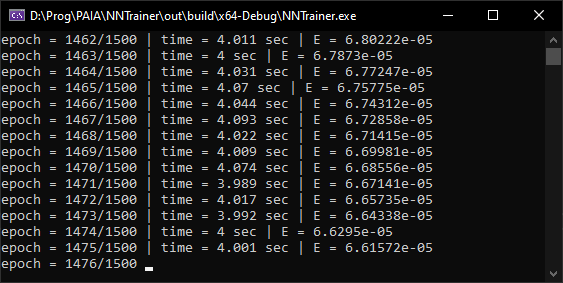
\includegraphics[width=120mm]{images/CurvedLerning.png}
    \caption*{\gostFont Рисунок \thechaptercntr .\theimagecntr \spc {--} Пример обучения нейронной сети в консоле}
    \label{fig:CurvedLerning}
  \end{figure} \addtocounter{imagecntr}{1}

  \par \redline В каждой строке определён номер эпохи, продолжительность эпохи и результат MSE. Построить кривую обучения можно взяв номера эпохи и соответствующие им значения MSE, но в консоли достаточно наблюдать за темпами ошибками. На этот темп влияет как гиперпараметры, так и сами данные которые были выбраны для обучения. В качестве обучающего набора были выбраны все данные третьего .csv файла, а в качестве контрольных данных выступают все данные 4-ого .csv файла. 

  \par \redline Пример кривых темпов обучения сети представлен на рисунке \thechaptercntr .\theimagecntr. На них сравнивалось пять моделей, у которх были некоторые общие гиперпараметры: скорость обучения $\alpha = 0.0001$, целевая ошибка $TE = 0.00001$, количество эпох $eps = 40$, выходная размерность $out = 4$, размер обущающего набора $TS = 200000$. На выход моделей нейронной сети подавались данные для прогнозирования температуры пастеризации. У моделей также различались и некоторые гиперпараметры, которые указаны в легенде графика.

  \par \redline Как можно увидеть на рисунке 4.6 больший эффект на обучение сети дёт входная размерность, нежели скрытая размерность. Строя таким образом графики кривых темпов обучения, каждый раз можно делать новый вывод, приблиющий к более эффективной конфигурации нейронной сети. 

  \par \redline Для определения качества модели нейронной сети используют кривые обучения {--} визуализация результатов оценки точности модели на этапе обучения модели нейронной сети и на этапе перекрёстной проверки, т.е. проверки на независимых данных. Пример этого представлен на рисунке \thechaptercntr .\theimagecntr.

  \begin{figure}[H]
    \centering
    \def\svgwidth{\textwidth}
    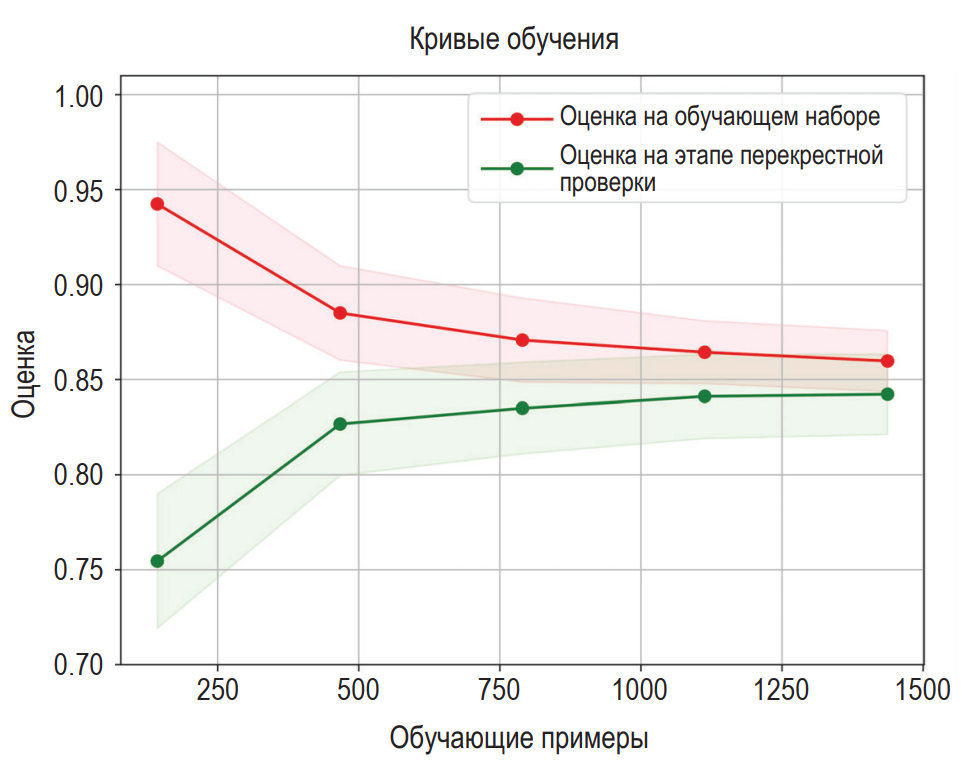
\includegraphics[scale=0.5]{images/CL.png}
    \caption*{\gostFont Рисунок \thechaptercntr .\theimagecntr \spc {--} Пример кривых обучения.}
    \label{fig:CL}
  \end{figure} \addtocounter{imagecntr}{1}

  \par \redline Кривые обучения также использовались при оценке модели нейронной сети. Однако гораздо показательнее будет визуализация результатов прогнозирования на данных тестового набора.

  \par \redline Результаты работ обученной модели нейронной сети для всех прогнозируемых параметров можно увидеть на рисунке ниже. На рисунке 4.6 изображено прогнозирование температуры пастеризации под действием степени открытия парового клапана в секции выдержки. На рисунке 4.7 изображено прогнозирование температуры гомогенизации под действием степени открытия парового клапана в секции подогрева. На рисунке 4.8 изображено прогнозирование расхода молока под действием мощности циркуляционного насоса.  

  \begin{sidewaysfigure}
    \centering
    \def\svgwidth{\textwidth}
    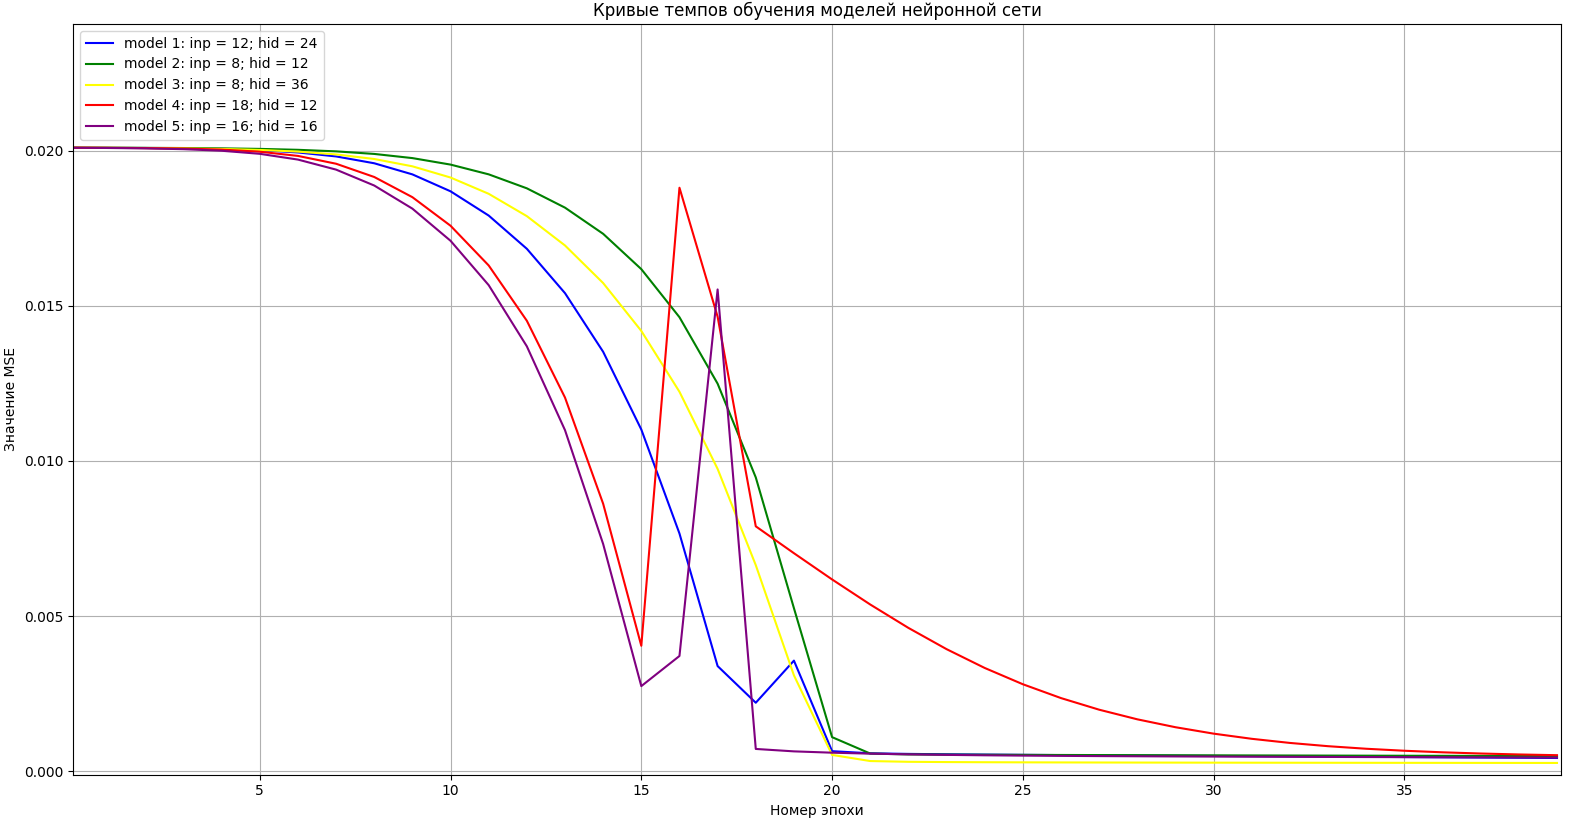
\includegraphics[width=\textheight]{images/CTL.png}
    \caption*{\gostFont Рисунок \thechaptercntr .\theimagecntr \spc {--} Пример визуализаци кривых темпов обучения.}
    \label{fig:CTL}
  \end{sidewaysfigure} \addtocounter{imagecntr}{1}

  \begin{sidewaysfigure}
    \centering
    \def\svgwidth{\textwidth}
    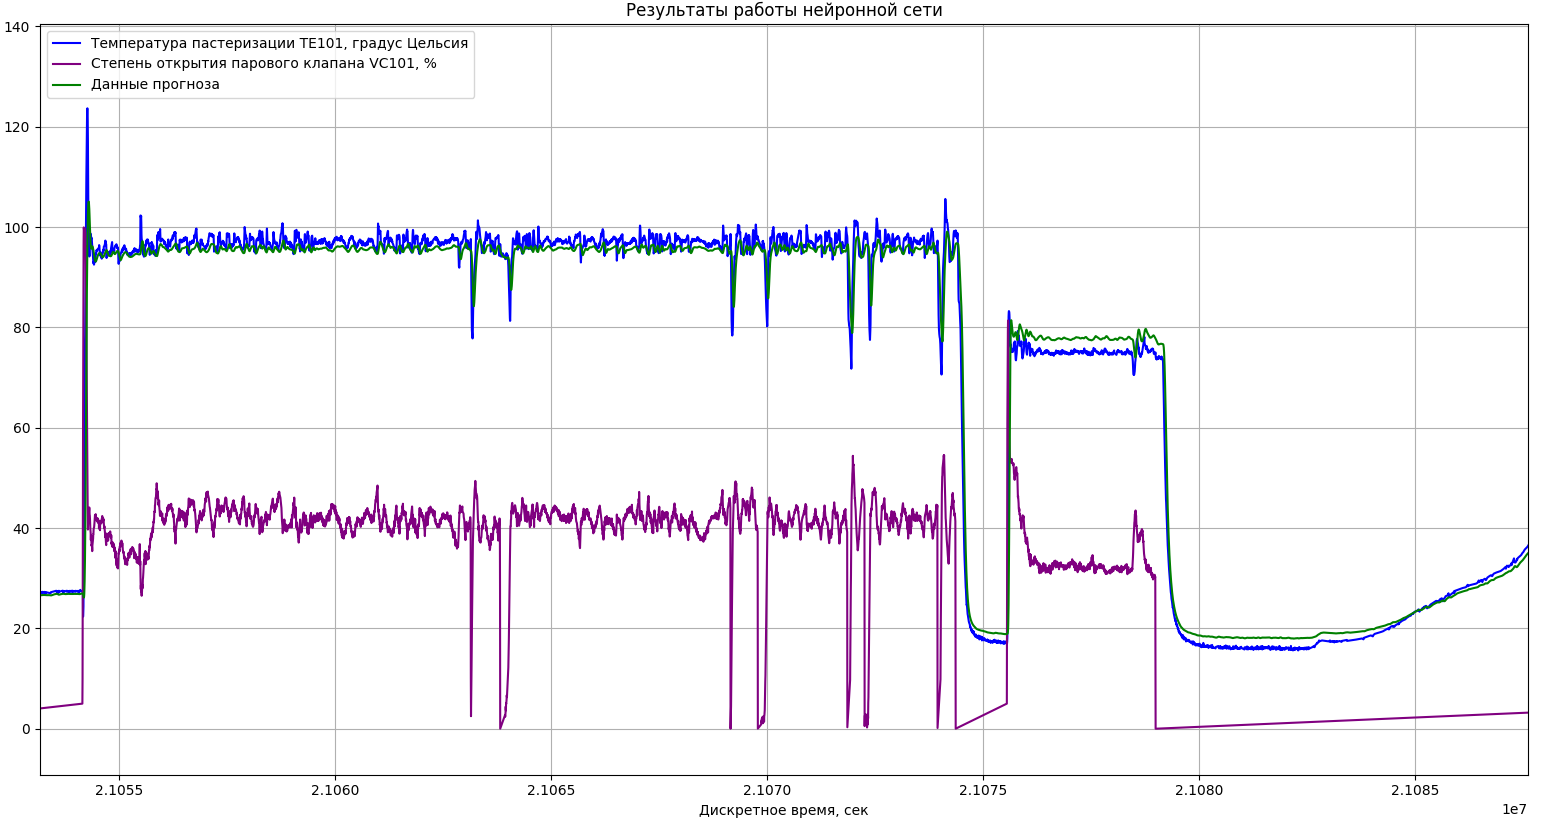
\includegraphics[width=\textheight]{images/TE101test.png}
    \caption*{\gostFont Рисунок \thechaptercntr .\theimagecntr \spc {--} Визуализация результатов прогнозирования температуры пастеризации.}
    \label{fig:TE101VisualPredict}
  \end{sidewaysfigure} \addtocounter{imagecntr}{1}

  \begin{sidewaysfigure}
    \centering
    \def\svgwidth{\textwidth}
    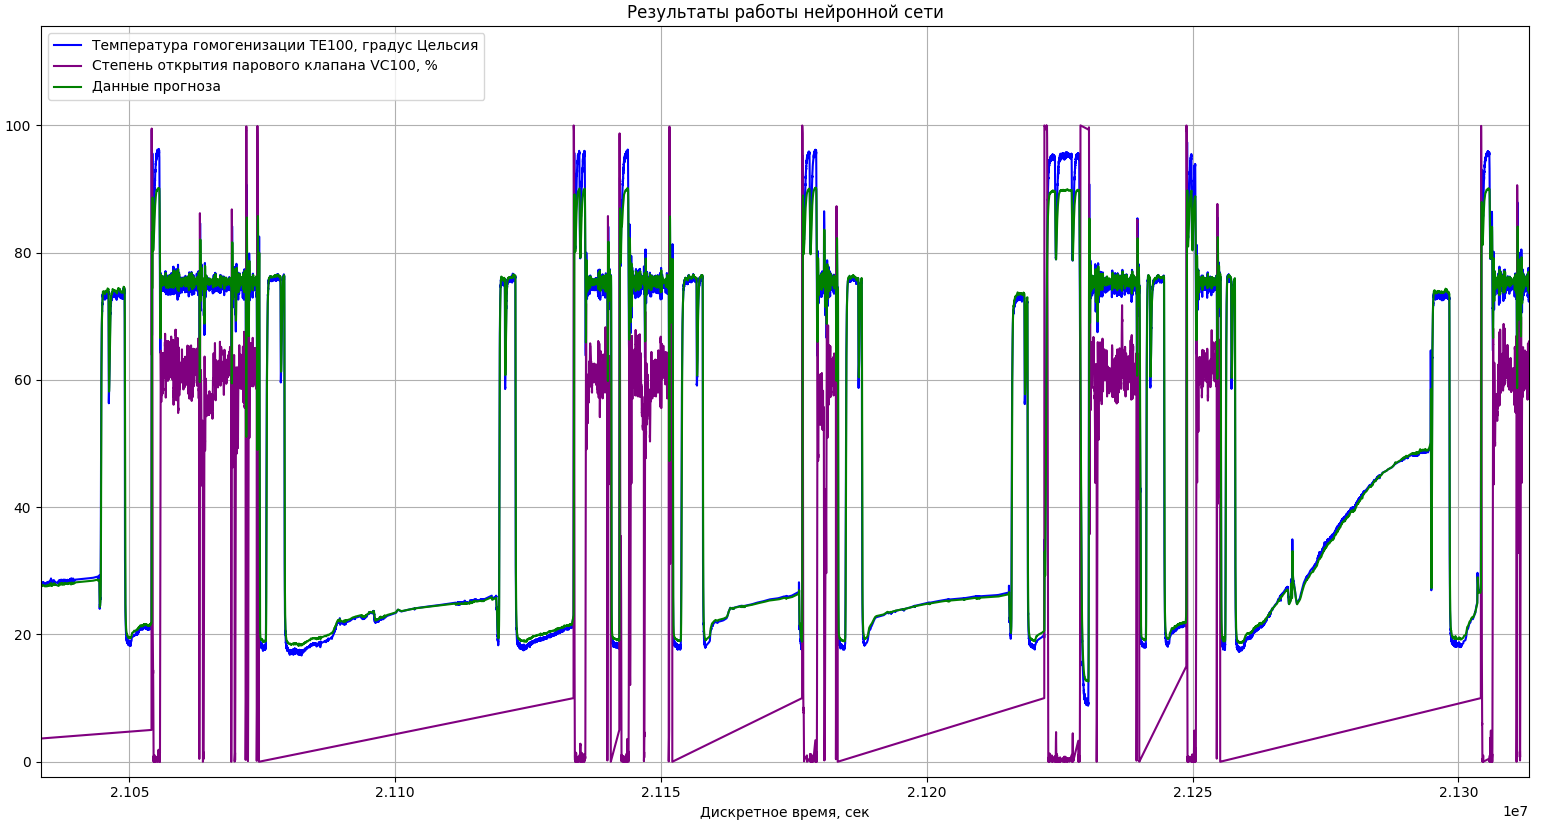
\includegraphics[width=\textheight]{images/TE100test.png}
    \caption*{\gostFont Рисунок \thechaptercntr .\theimagecntr \spc {--} Визуализация результатов прогнозирования температуры гомогенизации.}
    \label{fig:TE100VisualPredict}
  \end{sidewaysfigure} \addtocounter{imagecntr}{1}

  \begin{sidewaysfigure}
    \centering
    \def\svgwidth{\textwidth}
    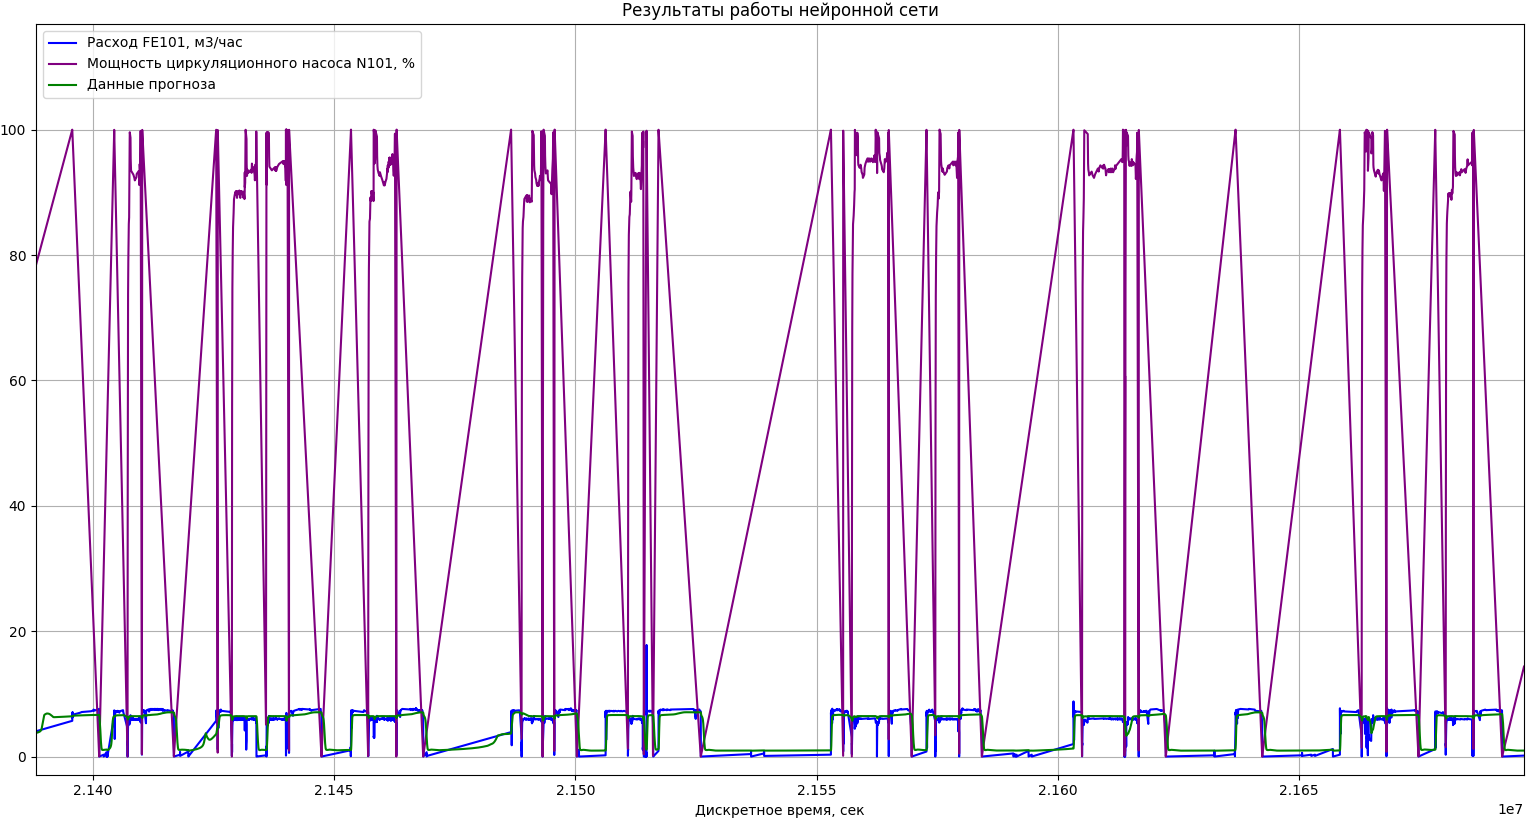
\includegraphics[width=\textheight]{images/FE101test.png}
    \caption*{\gostFont Рисунок \thechaptercntr .\theimagecntr \spc {--} Визуализация результатов прогнозирования расхода.}
    \label{fig:FE101VisualPredict}
  \end{sidewaysfigure} \addtocounter{imagecntr}{1}

}

\setcounter{subchaptercntr}{1}
\setcounter{formulacntr}{1}
\setcounter{imagecntr}{1}
